
The projections for anomalous coupling measurements from $\hzzllll$ decays at the HL-LHC were studied within the context of the last ECFA HL-LHC Experiments Workshops in 2013 and 2014~\cite{ATL-PHYS-PUB-2013-013}.
The obtained limits are quantified 
in terms of the effective couplings $g_i$  introduced in the invariant amplitude describing the interaction of a spin-0 particle and and two spin-one gauge bosons
introduced in Refs.~\cite{Gao:2010qx} and \cite{Heinemeyer:2013tqa}. The couplings $g_1$, $g_2$ and $g_3$ correspond to the 
interaction with the CP-even and $g_4$ to the interaction with the CP-odd boson, respectively.
The direct measurement of couplings is free of assumptions on the size of the interference effects and its results can be 
expressed in terms of the $(f_{g_i}, \phi_i)$ parametrisation:
%\begin{equation}
$$
f_{g_i} =\frac{|g_i|^2 \sigma _i ^2}{|g_1|^2 \sigma _1 ^2 + |g_2|^2 \sigma _2 ^2 + |g_4|^2 \sigma _4 ^2}; \;\;\; \phi _{g_i} = \arg \left ( \frac{g_i}{g_1} \right ).
$$
In this analysis $g_2$ and $g_4$ are measured separately, assuming the simultaneous presence of
only $g_1$ and of the coupling under study, this corresponds to set $g_2 = 0\; (g_4 = 0)$ in the expression of $f_{g_4}\;
( f_{g_2} )$ above.

The analysis was performed by fitting the observables based on the analytic calculation of Leading Order Matrix Element describing 
 $\hzzllll$ decays in the presence of anomalous couplings. The final fit is based on Monte Carlo modelling of the expected
signal at each bin of the $(\Re (g_i)/g_1; \Im (g_i) /g_1)$ plane, where $g_i$ represents $g_2$ or $g_4$. The irreducible $ZZ$ background 
 was suppressed by using a dedicated Boosted Decision Tree discriminant.  
 %A complimentary fit  approach has also been developed to compare results. The method implemented an eight-dimensional multivariate per-event extended likelihood, that makes full use of the available information and is therefore sensitive to both real and imaginary parts of the $g_i$ couplings. The likelihood is constructed by using the full analytical expression of the ME of the $\hzzllll$ process calculated at LO. Both approaches yielded very similar results.
 
%how the analysis was done
 
Following the event selection and applying the fit methodology described above, the expected exclusion
of the non-Standard Model contributions given the Standard Model data is evaluated for $300$ and $3000~\fbinv$.
Examples of the corresponding exclusion plots are given in Figure~\ref{fig:fgi-atlas-HZZ_anom_couplings}. With a conservative analysis limits of $f_{g_4} < 0.037$ at $95\%$~CL and 
$f_{g_2} < 0.12$ at $95\%$~CL for $3000~\fbinv$ are obtained. This allows a sensitive test of the tensor structure of the $\hzz$ couplings at the HL-LHC.

%%%%%%%%%%%%%%%%%%%%%%%%%%%%%
\begin{figure*}[!htbp]
\centering
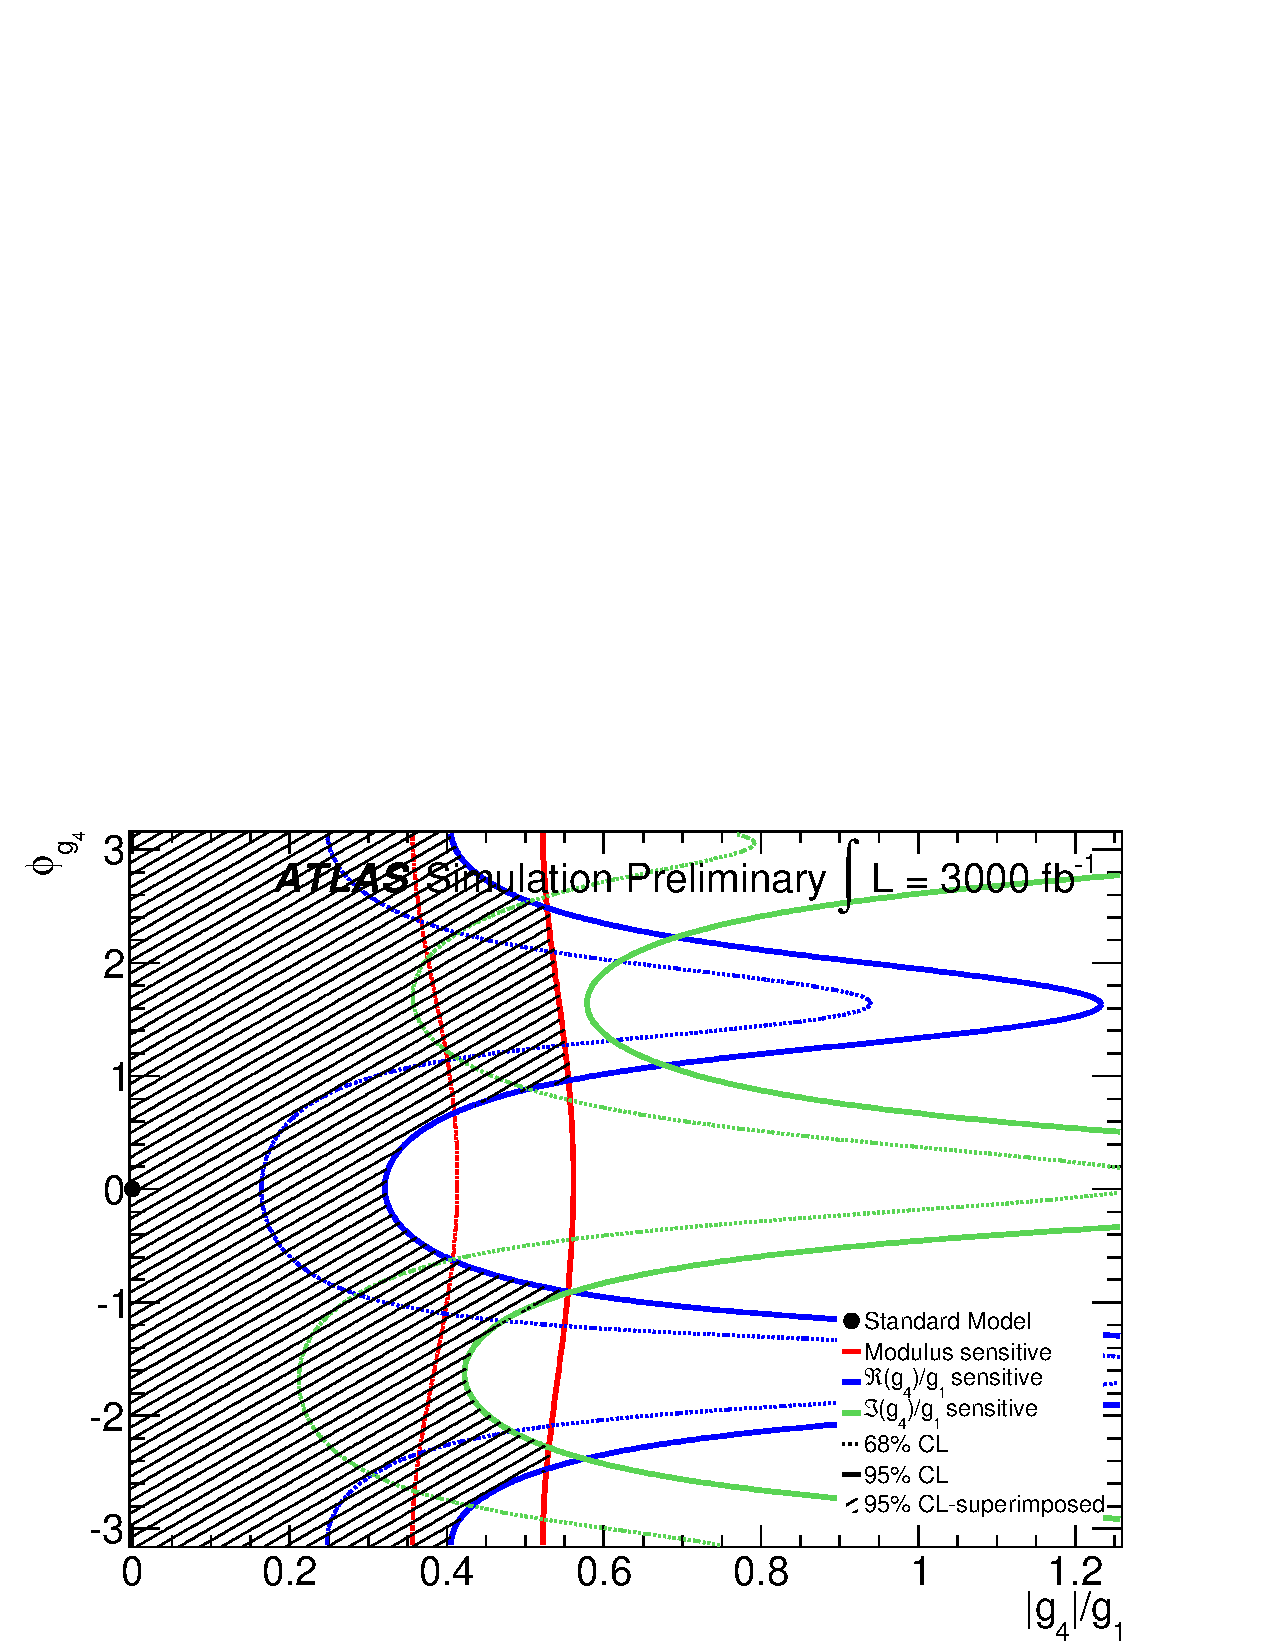
\includegraphics[width=0.70\textwidth]{section2/plots/hzz/ATL-PHYS-PUB-2013-013_fig_05d.pdf}
\caption
{
Results of the $g_4$-sensitive fits projected onto the ($|g_4|/g_1$, $\phi_{g_4}$) plane for $3000~\fbinv$. The shaded area corresponds to the most restrictive exclusion of the three observables. 
}
\label{fig:fgi-atlas-HZZ_anom_couplings}
\end{figure*}
%%%%%%%%%%%%%%%%%%%%%%%%%%%%%
